\section{Huffman-Codierung}

\begin{frame}
	Kann eine Codierung auch helfen, Zeichen zu sparen? \\
	\pause
	\impl Klar: \textbf{Komprimierung}!
\end{frame}

% too little time...
\only<beamer:0>{\xkcdframe{1683}{Digital Data}{2.5}}

\begin{frame}{Huffman-Codierungen}
	\begin{block}{Was ist das?}
		Eine \textbf{Huffman-Codierung} ist...
		\begin{itemize}
			\item ein präfixfreier Homomorphismus {\small (\impl einfach zu decodieren)}, sodass...
			\item Codierung eines Zeichens umso länger, je seltener das Zeichen vorkommt
		\end{itemize}
	\end{block}
	
	Die Huffman-Codierung für ein Wort ist dabei \textit{nicht eindeutig} (sehen wir gleich).
	\pause
	\begin{block}{Lemma}
		Unter allen präfixfreien Codes führen Huffman-Codes zu kürzesten Codierungen
		\textbf{des Wortes, für das die Huffman-Codierung konstruiert wurde.}
	\end{block}
\end{frame}

\begin{frame}{Konstruktionsverfahren}
	Kochrezept für einen Huffman-Baum zu einem geg. Wort:
	\begin{enumerate}
		\item Für jedes Zeichen die \emph{Häufigkeit} ermitteln
		\item Alle Zeichen mit ihrer Häufigkeit als \emph{Blätter} in die unterste Ebene zeichnen
		\item Nehme die zwei Knoten {\small (nicht unbedingt Blätter!)} mit \emph{geringsten Häufigkeiten} und lege einen Parent darüber an mit der Summe ihrer Häufigkeiten
		%\item Jeweils die zwei Knoten (nicht unbedingt Blätter!) mit den geringsten Häufigkeiten \enquote{verbinden}(also einen neuen Knoten darüber anlegen, der die Summe der Häufigkeiten erhält)
		\item Wiederhole (3), bis der ganze Baum aufgebaut ist.
		\item Die linken Äste mit \word 0 beschriften, die rechten Äste mit \word 1.
		\item Codierungen der Zeichen ablesen
		\item Ausgangswort codieren (wenn gefordert, nicht vergessen!)
	\end{enumerate}
\end{frame}

\begin{frame}{Beispiel}
	Gegeben: $w= \word{abadcadaac} $ (10 Zeichen) \\[1em]
	
	\only<1-3|handout:1>{ \visible<3>{
	\begin{minipage}{0.6\linewidth}
		\begin{figure}[b]
			\centering
			\begin{tikzpicture}
			[level 1/.style={sibling distance=40mm},
			level 2/.style={sibling distance=20mm},
			level 3/.style={sibling distance=15mm}]
			\node {$10$}
			child {
				node{$5$}
				child{
					node{$3$}
					child{
						node{$1,\word b$}
						edge from parent node[left] {\word 0}
					}
					child {
						node{$2,\word d$}
						edge from parent node[right] {\word 1}
					}
					edge from parent node[left] {\word 0};
				}
				child{
					node{$2,\word c$}
					edge from parent node[right] {\word 1}
				}
				edge from parent node[left] {\word 0\ \mbox{}};
			}
			child{
				node{$5,\word a$}
				edge from parent node[right] {\ \word 1}
			};
			\end{tikzpicture}
		\end{figure}  
	\end{minipage}
	}}
	\only<4-|handout:2> {
		\begin{minipage}{0.6\linewidth}
			Wie lang wird das codierte Wort $h(w)$?\\ \visible<5->{ 
			$5\*1 + 1\*3 + 2\*2 + 2\*3 = 18$ Zeichen\\ 
			Ähm, mehr Zeichen als vorher!? WTF? \\
			\visible<6->{\impl Keine Panik: \\
				Um ein Zeichen aus $\word a, \word b, \word c, \word d$ zu codieren, brauchen wir mindestens 2~Bit {\small (da 4 Möglichkeiten)}. \\ 
				Für die Zeichen $\word 0, \word  1$ brauchen wir aber nur ein Bit.  \\
				\impl 18 Bit statt 20 Bit \impl Platz gespart. \smiley
		}}
		\end{minipage}
	}
	\visible<2-> {
		\begin{minipage}{0.2\linewidth}
			\hfill
			\hfill 
			\vspace*{0.1\linewidth}
			\begin{table}[H]
				\begin{tabular}{c|cccc}
					\hline
					$x$ & \word a & \word b & \word c & \word d  \\ \hline
					$|w|_x$  & 5 & 1 & 2 & 2 \\ \hline
					$h(x)$ & \visible<3->{\word 1 & \word{000} & \word{01} & \word{001}} \\ \hline 
				\end{tabular}
			\end{table}
		\end{minipage}
	}
\end{frame}

\begin{frame}{Huffman-Codes}
		Huffman-Codierungen funktionieren immer nur gut für Wörter, die eine \textbf{ähnliche relative Zeichenhäufigkeit} haben wie das Wort, für das der Code erstellt wurde.
		\begin{Beispiel}
			$w_1 = \word{badcfehg}, \quad w_2 = \word a^1 \word b^2 \word c^4 \word d^8 \word e^{16} \word f^{32} \word g^{64} \word h^{128}$. \\
			Erstellt eine Huffman-Codierung für jedes Wort und codiert $w_1$ mit beiden Codierungen.\\
			Was verhalten sich die Längen der Codewörter?
			\visible<2->{
				\newcommand{\css}{\;\,}
				%\vspace{-.8\baselineskip}
				\begin{columns}[T] 
					\begin{column}[T]{.65\textwidth} 
							\begin{tabular}{c|c@{\css}c@{\css}c@{\css}c@{\css}c@{\css}c@{\css}c@{\css}c}
								\hline
								$x$ & \word a & \word b & \word c & \word d & \word e & \word f & \word g & \word h \\ \hline
								$|w_1|_x$  & 1 & 1 & 1 & 1 & 1 & 1 & 1 & 1 \\ \hline
								$h_1(x)$ & \word{000} & \word{001} & \word{010} & \word{011} & \word{100} & \word{101} & \word{110} & \word{111} \\ \hline 
							\end{tabular}
							\forcenewline\vspace{.3\baselineskip}
							\begin{tabular}{c|c@{\css}c@{\css}c@{\css}c@{\css}c@{\css}c@{\css}c@{\css}c}
								\hline
								$x$ & \word a & \word b & \word c & \word d & \word e & \word f & \word g & \word h \\ \hline
								$|w_2|_x$  & 1 & 2 & 4 & 8 & 16 & 32 & 64 & 128 \\ \hline
								$h_2(x)$ & $\word{1}^7$ & $\word{1}^6\word{0}$ & $\word{1}^5\word{0}$ & $\word{1}^4\word{0}$ & $\word{1}^3\word{0}$ & \word{110} & \word{10} & \word 0 \\ \hline 
							\end{tabular}
					\end{column}
					\hspace{-2\baselineskip}
					\begin{column}[T]{.35\textwidth} 
						\bigskip
						$\size{h_1(w_1)} = 8 \* 3 = 24$ \\
						$\size{h_1(w_2)} = 255 \* 3 = 765$ \\
						\bigskip
						\bigskip
						$\size{h_2(w_1)} = 35$ \\
						$\size{h_2(w_2)} = 501$
					\end{column}
				\end{columns}
				
			}
		\end{Beispiel}
\end{frame}


\begin{frame}{Huffman-Codes}
	\begin{block}{Erweiterung}
		Wir können nicht nur einzelne Buchstaben codieren. \\
		Bei $ w = \word a^{10} \word b^{10} \word c^{10} $ lohnt es sich, pro Block gleicher Buchstaben eine Codierung zu haben.
	\end{block}
\end{frame}


\subsection{Aufgaben}
\begin{frame}{Aufgabe (WS 2008) }
	Das Wort $$w = \word{0000\only<2->{\text{ }}0001\only<2->{\text{ }}0011\only<2->{\text{ }}0001\only<2->{\text{ }}0011\only<2->{\text{ }}0000\only<2->{\text{ }}0000\only<2->{\text{ }}1110\only<2->{\text{ }}0001\only<2->{\text{ }}0000}$$ soll komprimiert werden.
	
	\begin{itemize}
		\item[a)] Zerlegen Sie $w$ in Viererblöcke und bestimmen Sie die Häufigkeiten der vorkommenden Blöcke.
		\item[b)] Zur Kompression soll ein Huffman-Code verwendet werden. Benutzen Sie die in Teilaufgabe a) bestimmten Häufigkeiten, um den entsprechenden Baum aufzustellen. Beschriften Sie alle Knoten und Kanten.
		\item[c)] Geben Sie die Codierung des Wortes $w$ mit Ihrem Code an.
	\end{itemize}
\end{frame}

\begin{frame}{Lösung}
	$$w = \word{0000000100110001001100000000111000010000}$$
	\textit{a) Zerlegen Sie $w$ in Viererblöcke und bestimmen Sie die Häufigkeiten der vorkommenden Blöcke.} \\[1em]
	\pause
	$$w = \word{0000 0001 0011 0001 0011 0000 0000 1110 0001 0000}$$ \pause
	\begin{table}[h!]
		\centering
		\begin{tabular}{l|cccc}	
			& \word{0000} & \word{0001} & \word{0011} & \word{1110} \\ \hline
			Absolute Häufigkeiten: & 4 & 3 & 2 & 1 \\
			Relative Häufigkeiten:  & 0.4 & 0.3 & 0.2 & 0.1\\
		\end{tabular}
	\end{table}
\end{frame}

\begin{frame}{Lösung}
	\textit{b) Zur Kompression soll ein Huffman"=Code verwendet werden. Benutzen Sie die in Teilaufgabe a) bestimmten Häufigkeiten, um den entsprechenden Baum aufzustellen. Beschriften Sie alle Knoten und Kanten.}
	\begin{minipage}{0.45\linewidth}
		
		\pause 
		\begin{table}[h!]
			\centering
			\begin{tabular}{cccc}	
				\word{0000} & \word{0001} & \word{0011} & \word{1110} \\ \hline
				4 & 3 & 2 & 1 \\	
			\end{tabular}
		\end{table}
	\end{minipage}
	\hfill
	\begin{minipage}{0.5\linewidth}
		\begin{figure}[h!]
			\centering
			\visible<3>{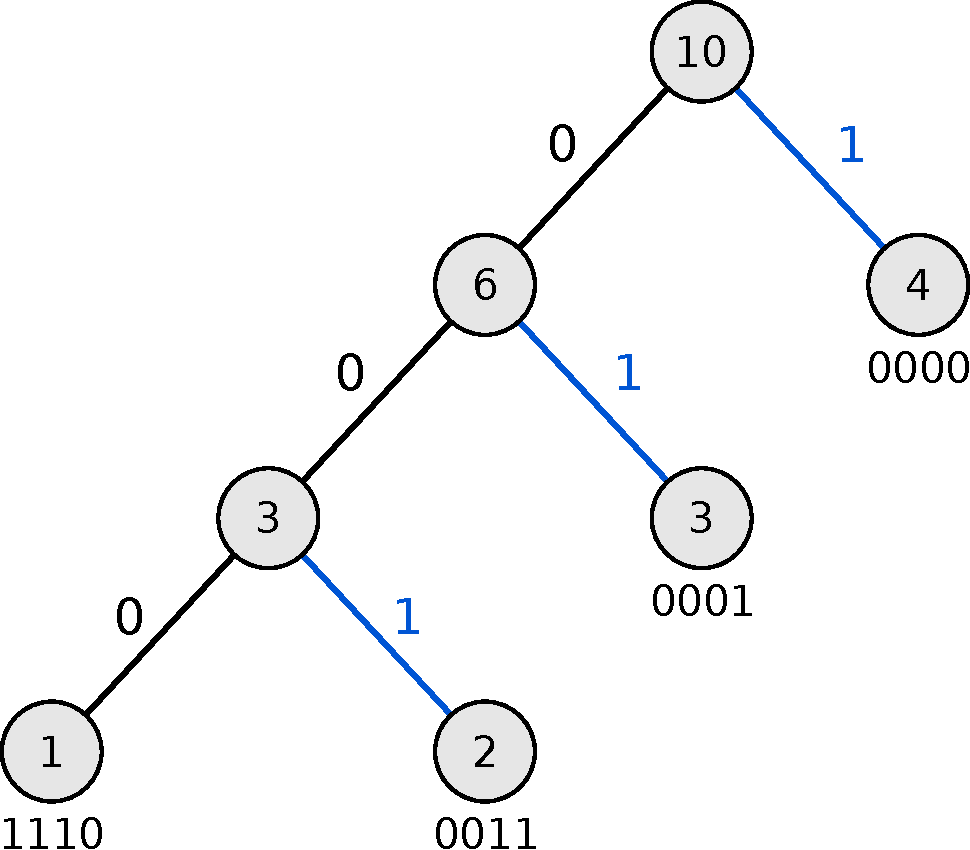
\includegraphics[scale=0.35]{Huffman.pdf}}
		\end{figure}
	\end{minipage}
\end{frame}

\begin{frame}{Lösung}
	\textit{c) Geben Sie die Codierung des Wortes $w$ mit Ihrem Code an.} \\[2em] \pause
	\begin{align*}
		h(&\word{0000000100110001001100000000111000010000}) = \\
		  &\word{1010010100111000011}
	\end{align*}
\end{frame}

%\begin{frame}
%	\frametitle{Aufgabe (WS 2010)}
%	Seien $n, k \in \N_0$ mit $1 \leq k \leq n$. In einem Wort $w \in \{a, b, c\}^\ast$ der Länge $3n$ komme $k$ mal das Zeichen $a$, $n$ mal das Zeichen $b$ und $2n - k$ mal das Zeichen $c$ vor.
%	\begin{itemize}
%		\item Geben Sie den für die Huffman-Codierung benötigten Baum an.
%		\item Geben Sie (in Abhängigkeit von $k$ und $n$) die Länge des zu $w$ gehörenden Huffman-Codes an.
%	\end{itemize}
%\end{frame}
%
%\begin{frame}
%	\frametitle{Lösung}
%	\vspace*{1em}
%	\begin{minipage}{0.45\linewidth}
%		\textit{$\dots$ Länge $3n$ komme $k$ mal das Zeichen $a$, $n$ mal das Zeichen $b$ und $2n - k$ mal das Zeichen $c$ vor. \\[1em] Geben Sie den für die Huffman-Codierung benötigten Baum an.} 
%		\pause
%		\begin{table}[h!]
%			\centering
%			\begin{tabular}{ccc}	
%				$a$ & $b$ & $c$ \\ \hline
%				$k$ & $n$ & $2n-k$ \\	
%			\end{tabular}
%		\end{table}
%		\pause
%		$$k \leq n \leq 2n -k $$ $$ n+k+2n-k = 3n$$
%	\end{minipage}
%	\hfill
%	\begin{minipage}{0.5\linewidth}
%		\begin{figure}[h!]
%			\centering
%			\only<4>{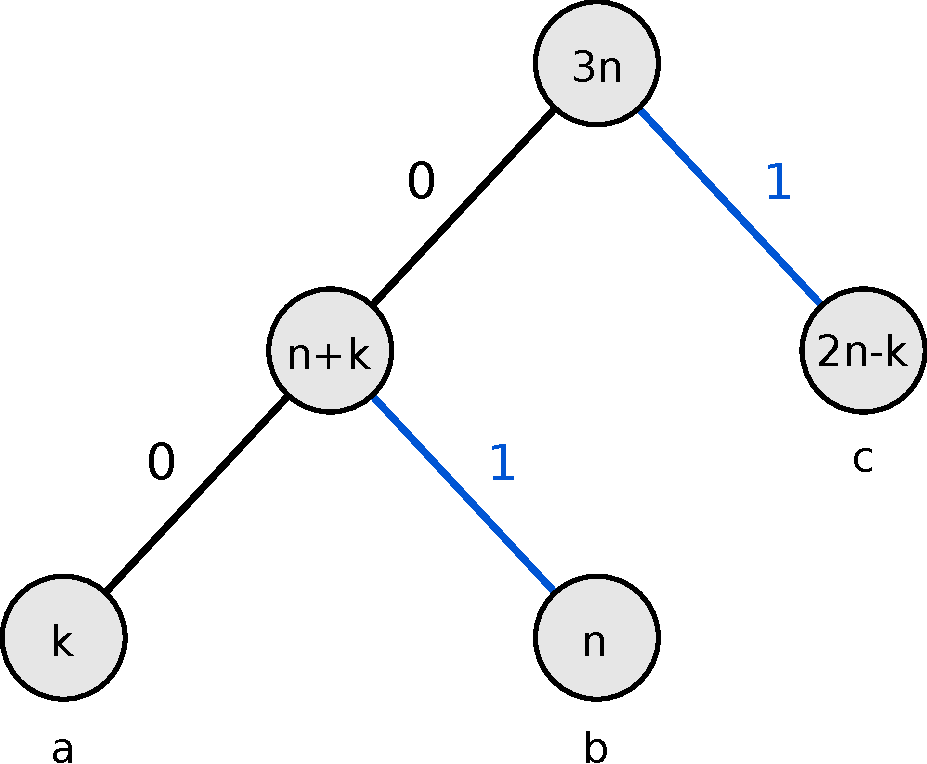
\includegraphics[scale=0.35]{Huffman2.pdf}}
%		\end{figure}
%	\end{minipage}
%\end{frame}
%
%\begin{frame}
%	\frametitle{Lösung}
%	\textit{Geben Sie die Länge des zu $w$ gehörenden Huffman-Codes an.} \\[2em]
%	\pause
%	Jedes $a$ und jedes $b$ wird durch zwei Zeichen codiert, und jedes $c$ wird durch ein Zeichen codiert. Damit erhält man insgesamt $$2k + 2n + 2n - k = 4n + k$$ Zeichen in der Codierung.
%\end{frame}


\begin{frame}{Ausblick}
	Die Huffman-Codierung hat ein Problem: Zum Decodieren muss der Huffman-Baum bekannt sein. Möglichkeiten:
	\begin{enumerate}
		\item Der Codebaum wird vor dem eigentlichen Codewort angegeben.\\ 
		\emph{Problem}: Das verlängert das Codewort.
		\item Es wird ein vorher festgelegter Codebaum verwendet.\\
		 \emph{Problem}: Dieser Codebaum kann evtl. sehr schlechte Ergebnisse liefern, da nicht für alle Wörter geeignet
	\end{enumerate}

	Diese Probleme können durch andere Codierungsverfahren gelöst werden, indem z.B. das Wörterbuch dynamisch während der Decodierung aus dem Codewort aufgebaut wird (z.~B. Lempel-Ziv-Welch-Verfahren).
\end{frame}

